\chapter{Booleovské obvody ($BO$)}

\section{Definície a označenia}

\begin{definicia}
Booleovký obvod je acyklický orientovaný graf, v ktorom vrcholy so vstupným stupňom 0
nazývame vstupné, vrcholy s výstupným stupňom 0 nazývame výstupné a vrcholom, ktoré nie
sú vstupné, sú priradené $\wedge$, $\vee$, $\neg$ (AND, OR, NOT). Vstupné vrcholy označím
$x_1, x_2, ..., x_k$ alebo $0$ alebo $1$
\end{definicia}

Booleovský obvod počíta funkciu $f: B^n \rightarrow B^m$, kde $n$ je počet vstupných a
$m$ výstupných vrcholov. Štandardne platí, že AND a OR má 2 vstupy a NOT jeden. My budeme
v nasledujúcom uvažovať, že booleovský obvod má len jeden výstup, keďže obvod s $m$
výstupmi sa dá "rozbiť" na m obvodov, ktoré majú len jeden výstup.\\ Je rozumné zamyslieť
sa, kedy bude na výstupe booleovského obvodu platný výsledok. Ak uvažujeme, že prechod
vrcholom nám trvá jednu časovú jednotku (po hrane je to zadarmo), po čase rovnom
najdlhšej ceste v grafe už určite bude na výstupe korektný výsledok.

\begin{definicia}
Definujeme jazyky pomocou obvodov:\\ Jazyk generovaný triedou obvodov
$\{C_n\}_{n=0}^{\infty}$, kde $C_n$ má $n$ vstupných vrcholov označených\\ $x_1,...,x_n$
a jeden výstupný vrchol, je $L(\{C_n\}_{n=0}^{\infty})=\{w \in \{0,1\}^* \mm $Obvod
$C_{|w|}$ pri vstupe $a_1,...,a_{|w|}$, kde $w=a_1...a_{|w|}$, má hodnotu výstupu $1\}$
\end{definicia}

Booleovské obvody sú neuniformný model, lebo pre každú dĺžku vstupu môže byť iný obvod.

\begin{definicia}
Uniformné booleovské obvody sú také obvody $\{C_n\}_{n=0}^{\infty}$, pre ktoré existuje
deterministický TS, ktorý na vstupe $1^n$ (teda na vstupe obsahujúcom $n$ jednotiek)
"vyrobí" obvod $C_n$
\end{definicia}

To nám zaručuje, že nemôžem vybehnúť mimo rekurzívne vyčísiteľné jazyky.

\section{Kódovanie Booleovských obvodov}

Booleovské obvody bodeme kódovať takto: Jednotlivým vrcholom priradíme identifikátor -
číslo. Vrcholy $x_1,x_2,...,x_k$ budú mať identifikátory 1,2,...,k. Kód obvodu $C_n$
(označujeme $\langle C_n \rangle$) bude postupnosť štvoríc: (číslo vrchola, funkcia,
číslo ľavého vstupu, číslo pravého vstupu), kde funkcia je z množiny $\{\wedge , \vee ,
\neg , 0 , 1 , vstup \}$\footnote{$0,1$ nám označujú booleovské konštanty}\\ Tu sa
dohodneme, že vrchol s číslom 0 označuje výstup.\\ O topologickom usporiadaní hovoríme
vtedy, keď vrchol sa objaví v kóde až vtedy, keď tam už boli jeho vstupy.

\section{Miery zložitosti pre booleovské obvody}

Pre booleovské obvody definujeme nasledujúce miery zložitosti:
\begin{itemize}
\item{SIZE($C_n$) }označuje počet hradiel (okrem vstupných vrcholov) obvodu $C_n$
\item{DEPTH($C_n$) }charakterizuje dĺžku najdlhšej cesty v obvode
\end{itemize}

\begin{priklad}
Skalárny súčin dvoch booleovských vektorov vypočítame takto:\\ $(x_1, x_2, ..., x_n) .
(y_1, y_2,..., y_n)=\underset{i=1}{\overset{n}\bigvee}(x_i\wedge y_i)$

\begin{figure}[!ht]
\centering
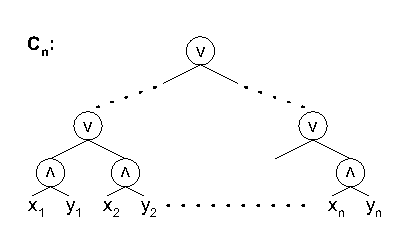
\includegraphics{img/bobr1}
\caption{} \label{BObr1}
\end{figure}

\begin{itemize}
\item DEPTH($C_n$)$=\log_2n$
\item SIZE($C_n$)$=2n-1=O(n)$
\end{itemize}

Ukážme si, ako inak môžme skonštruovať obvod na výpočet skalárneho súčinu:

\begin{figure}[!ht]
\centering
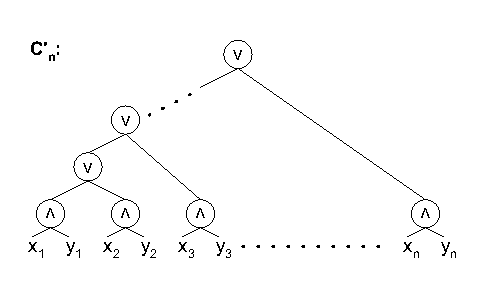
\includegraphics{img/bobr2}
\caption{} \label{BObr2}
\end{figure}

\begin{itemize}
\item DEPTH($C'_n$)$=O(n)$
\item SIZE($C'_n$)$=O(n)$
\end{itemize}

Tu vidíme že aj napriek tomu, že sa nám zväčšila hĺbka, nedokázali sme zmenšiť počet
hradiel.\\ Pre zaujímavosť: $|\langle C_n \rangle | =$SIZE($C_n$)$*\log$ SIZE($C_n$) lebo
jedno hradlo dokážeme zapísať na priestor veľkosti $\log$ SIZE($C_n$) a počet hradiel je
SIZE($C_n$)

\end{priklad}

\begin{priklad}
Násobenie matíc: je to $n^2$ skalárnych súčinov, každý z nich sa robí nezávisle, teda
podľa predchádzajúceho príkladu platí:

\begin{itemize}
\item DEPTH($C_n$)$=\log_2n$
\item SIZE($C_n$)$=n^2*O(n)=O(n^3)$
\end{itemize}

\end{priklad}

\begin{priklad}\label{Priklad1}
Tranzitívny reflexívny uzáver booleovskej matice M:\\ $M^*=I\vee M\vee M^2 \vee ...\vee
M^n=(I\vee M)^n$, kde $M^i=\underbrace{M\wedge M\wedge ... \wedge M}_{i}$ \\ Ideme len po
$M^n$ preto, lebo ostatné sa už opakujú.

\begin{figure}[!ht]
\centering
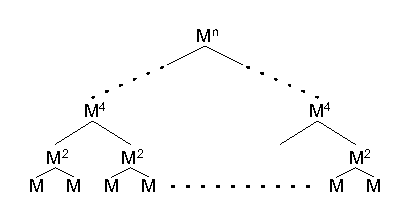
\includegraphics{img/bobr3}
\caption{} \label{BObr3}
\end{figure}

Z obrázku \ref{BObr3} a predchádzajúceho príkladu vyplýva, že
\begin{itemize}
\item DEPTH($C_n$)$=O(\log^2n)$
\item SIZE($C_n$)$=n*O(n^3)=O(n^4)$
\end{itemize}

\end{priklad}

\section{Simulácie TS a BO}

\begin{veta}
Ak $L$ je akceptovaný deterministickým 1-páskovým TS - A v čase T(n), potom $L$ sa dá
definovať postupnosťou BO $\{C_n\}_{n=0}^{\infty}$ takých, že SIZE($C_n$)$=O(T^2(n))$
\end{veta}

\begin{dokaz}(Zatiaľ nekompletný) Zapíšeme konfigurácie TS pri výpočte na slove
$a_1a_2...a_n$\\ do "tabuľky":
\begin{center}
\begin{tabular}{rcccccc}

   koncová konfigurácia:& $c_1$    &  $c_2$   & $...$ & $c_n$  & $...$ & $c_m$ \\

                        & $...$    &          &       &     \\

konfigurácia po 1.kroku:& $b_1$    & $q_1a_2$ & $...$ & $a_n$     \\

počiatočná konfigurácia:& $q_0a_1$ & $a_2$    & $...$ & $a_n$     \\

\end{tabular}
\end{center}
kde počet stĺpcov tabuľky, ako aj počet riadkov je rovný T(n). $q_0a_1$, ako aj $q_1a_2$
a ďalšie také, prehlásime za jeden symbol. Ak si očíslujeme riadky zdola hore číslami
1,2,...,k a stĺpce zľava doprava číslami 1,2,...,l , tak obsah políčka (i,j) môžu
ovplyvniť len políčka (i-1,j-1), (i-1,j) a (i-1,j+1) (Obrázok\ref{BObr4}) .
\begin{figure}[!ht]
\centering
%\includegraphics{img/BObr4}
\caption{CHÝBA OBRÁZOK} \label{BObr4}
\end{figure}

Políčko bude vyzerať takto: \begin{tabular}{|c|c|} \hline 1011 & 0101 \\ \hline
\end{tabular}, kde v prvej časti je kód stavu (ak je tam 00...0 znamená to, že nie je tam
stav) a v druhej časti je kód znaku.

\end{dokaz}

\begin{veta}
Nech A je NTS so vstupnou páskou a jednou pracovnou páskou a vstupnou abecedou
$\Sigma=\{0,1\}$. Ak A akceptuje slová dĺžky n v priestore $S(n)\geq \log\med n$, potom
existuje booleovský obvod hĺbky $\approx S^2(n)$, ktorý akceptuje slová dĺžky n z $L(A)$
\end{veta}

\begin{dokaz}
Keďže máme ohraničený priestor, tak vieme, že A môže byť v maximálne $k^{S(n)}$
konfiguráciách pre nejakú konštantu $k$. Môžeme predpokladať, že A má jednoznačne
danú\footnote{čiže jedinú jednu} akceptačnú konfiguráciu. Nech $\vdash$ je relácia na
konfiguráciách. Keďže konfigurácii je $k^{S(n)}$, je $\vdash$ konečná relácia definovaná
booleovskou maticou veľkosti $k^{S(n)}\times k^{S(n)}$.\\ Otázka, či $w\in L$, je otázka,
či počiatočná konfigurácia na $w$ je v relácii $\overset{*}\vdash$ \footnote{tiež je
konečná, tiež sa dá reprezentovať booleovskou maticou $k^{S(n)}\times k^{S(n)}$}s
akceptačnou konfiguráciou.\\ Tranzitívny a reflexívny uzáver relácie $\vdash$ vieme podľa
príkladu \ref{Priklad1} získať obvodom hĺbky $\log^2(k^{S(n)})$, čo je zhruba $S^2(n)$.
\end{dokaz}

\begin{definicia}
Postupnosť booleovských obvodov $\{C_n\}_{n=0}^{\infty}$ je BC - uniformne
konštruovateľná, ak existuje deterministický TS, ktorý pre každé n na vstupe $1^n$
vypočíta kód obvodu $C_n$ v priestore $\log(SIZE(C_n))$
\end{definicia}

Ako vyzerá DTS:

\begin{figure}[!ht]
\centering
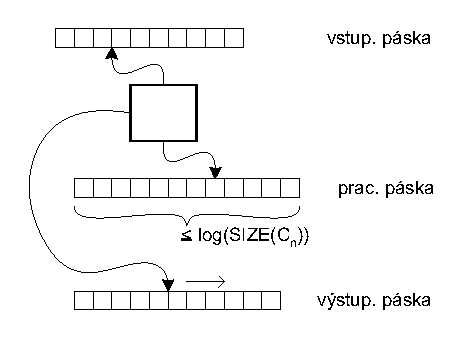
\includegraphics{img/bobr5}
\caption{} \label{BObr5}
\end{figure}

\begin{description}
\item $SIZE(C_n)$ - maximálny čas na pracovnej páske
\item $SIZE(C_n).\log(SIZE(C_n))$ - veľkosť výstupu (a teda aj čas)
\end{description}

- o čase vieme povedať: $SIZE(C_n).\log(SIZE(C_n))$ - z obmedzenia DTS

\begin{oznacenie}
$\mathcal{U}_{BC}SIZE \med DEPTH(S(n),D(n))$ je trieda jazykov, pre ktoré existuje
postupnosť booleovských obvodov veľkosti $\approx S(n)$ a hĺbky $\approx D(n)$
\end{oznacenie}

\begin{veta}\label{Veta1}
$L\in \mathcal{U}_{BC}Size(S(n))$ potom $L\in DTIME(Poly(S(n)))$
\end{veta}

\begin{dokaz}
\begin{enumerate}
\item Nech $A$ je DTS, ktorý vyrába obvod $C_n$ v prietore $\log(SIZE(C_n))$. Zostrojíme DTS
$A'$, ktorý vyrobí na pracovnej páske kód $C_n$ simulovaním $A$ - to vieme v čase
$[S(n)*\log(S(n))]$, čo je aj maximálna veľkosť pracovnej pásky
\item Postupne priraďujeme hodnoty jednotlivým vrcholom $C_n$. Vstupným podľa vstupného
slova, ostatným podľa hodnôt predchodcov. Keďže pre každý vrchol musím prebehnúť pásku a
mám $S(n)$ vrcholov, teda výsledný čas DTS $A'$ bude približne $[S(n)*S(n)*\log(S(n))]$,
čo je polynomiálna veľkosť.
\end{enumerate}
\end{dokaz}

\begin{veta}\label{Veta2}
$L\in \mathcal{U}_{BC}DEPTH(D(n))$ potom $L\in DSPACE(D(n))$
\end{veta}

\begin{dokaz}
Zrejme $D(n)\geq \log(SIZE(C_n))$, lebo najviac hradiel v určitej hĺbke je v úplnom
binárnom strome. Čiže v priestore $D(n)$ vieme simulovať konštruktor kódu obvodu $C_n$.
Obvod budeme vyhodnocovať postorder prehľadávaním obvodu $C_n$. Pritom budeme opakovane
generovať kódy jednotlivých vrcholov podľa toho, ktorý vrchol budeme práve potrebovať
(lebo kód celého obvodu sa nám nevmestí do priestoru $D(n)$). Taktiež si musíme nejakým
spôsobom pamätať, kde v strome sa nachádzame (navigáciu). Keby sme si navigáciu pamätali
ako kódy všetkých vrcholov po ktorých sme šli, mohlo by to v najhoršom prípade zabrať
veľmi veľa priestoru. Preto si budeme pamätať len navigačný reťazec(napríklad:0,0,1,...
kde 0=vľavo a 1=vpravo).\\ - z časového hľadiska je to veľmi neefektívna simulácia, keďže
zakaždým od začiatku generujeme kódy vrcholov ktoré momentálne potrebujeme, ale
nepresiahneme priestor $D(n)$
\end{dokaz}

\begin{dosledok}
$PSPACE(\equiv DSPACE(Poly)=NSPACE(Poly))=\mathcal{U}_{BC}DEPTH(n^{O(1)})$
\end{dosledok}

\begin{definicia}
Model počítača patrí do triedy počítačov druhej triedy, ak sekvenčný nedeterministický
priestor je v polynomiálnom vzťahu s časom na danom modeli (jeden bol alternujúci stroj a
druhý booleovský obvod)
\end{definicia}

Rýchlo paralelne počítateľné problémy - problémy, ktoré sa dajú počítať na nie príliš
hlbokých a nie príliš košatých obvodoch (polylogaritmická hĺbka a polynom. veľkosť).

\begin{definicia}
(Nick's Class)
\begin{description}
\item $\mathcal{NC}^i = \mathcal{U}_{BC}SIZE \med DEPTH(n^{O(1)},\log^in)$
\item $\mathcal{NC} = \underset{i\geq 1}\bigcup \mathcal{NC}^i$
\end{description}
\end{definicia}

\begin{veta}
$\mathcal{NC} \subseteq P $
\end{veta}

\begin{dokaz}
Vyplýva z vety \ref{Veta1}
\end{dokaz}

Otvoreným problémom je rovnosť $\mathcal{NC}$ a $P$. Predpokladá sa ale, že podobne ako
pre $P$ a $NP$, aj tu platí: $\mathcal{NC}\neq P$

\begin{veta}
$\mathcal{NC}^i \subseteq DSPACE(\log^in)$
\end{veta}

\begin{dokaz}
Vyplýva z vety \ref{Veta2}
\end{dokaz}

\begin{dosledok}
$\mathcal{NC} \neq PSPACE$
\end{dosledok}

\begin{poznamka}
Vieme: $\mathcal{NC} \subseteq P \subseteq NP \subseteq PSPACE$, ale nevieme, kde je
porušená súvislosť
\end{poznamka}

\begin{priklad}
$L=\{ww^R\mm w\in \{0,1\}^* \} \in \mathcal{NC}^1$\\  Na obrázku \ref{BObr6} je
znázornený obvod pre daný jazyk $L$. Ekvivalencia sa pomocou $\{\wedge,\vee,\neg\}$ dá
napísať napríklad takto: $a\equiv b \Leftrightarrow (a\wedge b)\vee(\neg a \wedge \neg
b)$.
\end{priklad}

\begin{figure}[!ht]
\centering
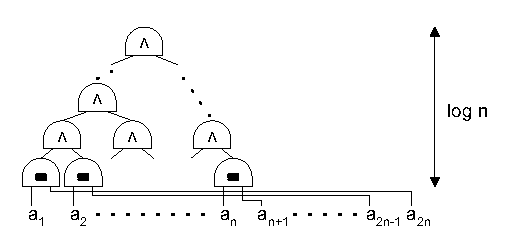
\includegraphics{img/bobr6}
\caption{} \label{BObr6}
\end{figure}


Ak počítame funkcie, uvažujeme triedu funkcií $\mathcal{FNC}$\\ Násobenie matíc je v
$\mathcal{FNC}^1$ - hĺka je logaritmická, veľkosť polynomiálna. \\ Tranzitívny a
reflexívny uzáver je v $\mathcal{FNC}^2$ - hĺbka je $\log^2$. \\ - trieda $\mathcal{NC}$
(na rozdiel od $\mathcal{NC}^i)$ je dosť odolná voči uniformitám.

\section{Ďalšie druhy uniformity}

\begin{definicia}
Majme danú postupnosť booleovských obvodov $\{C_n\}_{n=0}^\infty$. Jej príslušný
rozšírený jazyk prepojení je nasledujúci jazyk: $L_e = \{\langle n,g,p,y\rangle \mm n,g
\in \{0.1\}^*;\med p \in \{L,R\}^*;\\ |p|\leq \log(SIZE(C_n));\med y\in \{\times, \wedge,
\vee, \neg\}\cup \{0,1\}^*$\footnote{$\times$ označuje vstupné hradlo}, pričom v obvode
$C_n$ platí jedna z vecí:
\begin{description}
\item{(i) }$p=\varepsilon$ a hradlo číslo g je typu y
\item{(ii) } $p\neq \varepsilon$ a hradlo $g(p)$ má číslo y $\}$
\end{description}
\begin{description}
\item $g(L)$ je ľavý vstup hradla g
\item $g(R)$ je pravý vstup hradla g
\item $g(Lw)=(g(L))w$
\item $g(Rw)=(g(R))w$
\end{description}
\end{definicia}

\begin{priklad}
Rozšírený jazyk prepojení, ktorého obvod $C_4$ je znázornený na Obr \ref{BObr7} vyzerá
takto:\\
$L_e=\{\underbrace{\med\med\med\med\med\med\med\med\med\med}_{C_1,C_2,C_3}\med,\overset{x_1}{\langle
1111,1,\varepsilon,\times \rangle},\overset{x_2}{\langle 1111,10,\varepsilon,\times
\rangle},\overset{x_3}{\langle 1111,11,\varepsilon,\times \rangle}, \overset{x_4}{\langle
1111,100,\varepsilon, \times \rangle},\\ \overset{\mbox{\scriptsize 1.možnosť
č.5}}{\langle 1111,101,\varepsilon, \wedge \rangle },\overset{\mbox{\scriptsize 2.možnosť
č.5}}{\langle 1111,101,L, 1 \rangle },\overset{\mbox{\scriptsize 3.možnosť č.5}}{\langle
1111,101,R, 10 \rangle },...,\overset{\mbox{\scriptsize 1.možnosť č.8}}{\langle
1111,1000,\varepsilon, \vee \rangle }, \overset{\mbox{\scriptsize 2.možnosť č.8}}{\langle
1111,1000,L, 111 \rangle },\\ \overset{\mbox{\scriptsize 3.možnosť č.8}}{\langle
1111,1000,R, 100 \rangle },\overset{\mbox{\scriptsize 4.možnosť č.8}}{\langle
1111,1000,LL, 101 \rangle },\overset{\mbox{\scriptsize 5.možnosť č.8}}{\langle
1111,1000,LR, 110 \rangle },\overset{\mbox{\scriptsize 6.možnosť č.8}}{\langle
1111,1000,LRL, 10 \rangle },...\}$

\end{priklad}

\begin{figure}[!ht]
\centering
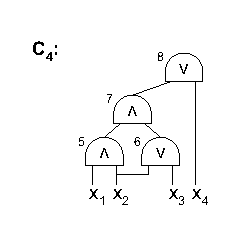
\includegraphics{img/bobr7}
\caption{} \label{BObr7}
\end{figure}

\begin{definicia}\label{Def1}
Postupnosť booleovských obvodov $\{C_n\}_{n=o}^{\infty}$ veľkosti $S(n)$ a hĺbky $D(n)$
je
\begin{description}
\item{(a) }$\mathcal{U}_E$ - uniformná, ak existuje DTS, ktorý akceptuje $L_e$ tak, že
slová $\langle n,...\rangle$\footnote{ktoré popisujú n-ty obvod} akceptuje v čase
$\log(S(n))$
\item{(b) }$\mathcal{U}_{E^*}$ - uniformná, ak existuje ATS akceptujúci $L_e$ tak, že
slová $\langle n,...\rangle$ akceptuje v čase $D(n)$ a priestore
$\log(S(n))$\footnote{implicitne predpokladáme, že máme obvody očíslované, pričom
nepoužívame veľmi veľké čísla}
\end{description}
\end{definicia}

\begin{lema}\label{Lema1}
Nech je daná postupnosť booleovských obvodov $\{C_n\}_{n=0}^{\infty}$ veľkosti $S(n)$.
Nech $f(n)=\Omega (\log(S(n)))$. Potom $(1)$ štandardný kód obvodu $C_n$ sa dá vypočítať
v $DSPACE(f(n)) \Leftrightarrow \med (2) \med L_e \widetilde{\in}$\footnote{priestor
$f(n)$ na slovách $\langle n,...\rangle$}$DSPACE(f(n))$
\end{lema}

\begin{dokaz}
\begin{description}
\item{$(1)\Rightarrow (2)$ }Na zistenie, či $\langle n,g,p,y \rangle \in L_e$ budeme robiť
nasledujúcu vec:
\begin{description}
\item{(i) }Budeme simulovať generátor kódu pre obvod $C_n$, kým nevyrobí $(g,t,a,b)$
\item{(ii) }Overíme typ: ak $p=\varepsilon$: akceptuj ak $y=t$, inak $reject$
\item{(iii) }Rekurzívne overíme číslo:
\begin{description}
\item ak $p=Lp'$:
\begin{description}
\item ak $p'=\varepsilon$ akceptuj ak $y=a$
\item ak $p'\neq \varepsilon$ akceptuj ak $y=a(p')$\footnote{rekurzívne vytvorí
$(a,.,.,.)$ a overuje}
\end{description}
\item ak $p=Rp'$:
\begin{description}
\item ak $p'=\varepsilon$ akceptuj ak $y=b$
\item ak $p'\neq \varepsilon$ akceptuj ak $y=b(p')$
\end{description}
\end{description}
\end{description}
\item{$(2)\Rightarrow (1)$ }Štandardný kód pre obvod $C_n$ budeme generovať takto:
\begin{description}
\item{(i) }Zistíme najväčšie číslo hradla v obvode $C_n$\footnote{predpokladám
číslovanie "bez dier"} \\ $g_{max}$ získam tak, že postupne testujem pre $g=0,1,2,...$ a
$t\in \{\times, \wedge, \vee, \neg\}$, či $\langle n,g,\varepsilon, t\rangle \in L_e$,
kým existuje také $t$
\item{(ii) }Pre každé $g=0,1,...,g_{max}$ vyrobíme štvoricu $(g,t,g_L,g_R)$ tak, že $g_L$
resp. $g_R$ nájdeme testovaním $\langle n,g,L,h \rangle \forall h \in
\{0,1,...,g_{max}\}$ resp. $\langle n,g,R,h \rangle \forall h \in \{0,1,...,g_{max}\}$ a
typ testujem tak, že testujem $\langle n,g,\varepsilon,t \rangle$ pre $t\in
\{\times,\wedge,\vee,\neg \}$
\end{description}
\end{description}
\end{dokaz}

\section{Vzťahy uniformít}

\begin{veta}
Platia nasledujúce vzťahy uniformít:
\begin{enumerate}
\item $\{C_n\}_{n=0}^{\infty}$ je $\mathcal{U}_E$ - uniformná $\Rightarrow$
$\{C_n\}_{n=0}^{\infty}$ je $\mathcal{U}_{BC}$ - uniformná
\item $\{C_n\}_{n=0}^{\infty}$ je $\mathcal{U}_E$ - uniformná $\Rightarrow$
$\{C_n\}_{n=0}^{\infty}$ je $\mathcal{U}_{E^*}$ - uniformná
\item Ak $D(n)\geq \log^2(S(n))$, potom \\ $\{C_n\}_{n=0}^{\infty}$ je
$\mathcal{U}_{BC}$ - uniformná $\Rightarrow$ $\{C_n\}_{n=0}^{\infty}$ je
$\mathcal{U}_{E^*}$ - uniformná
\end{enumerate}
\end{veta}

\begin{dokaz}

\begin{enumerate}
\item Ak $\{C_n\}_{n=0}^{\infty}$ je $\mathcal{U}_E$ - uniformná
$\overset{Def.\ref{Def1}}{\Longrightarrow} L_e \widetilde{\in} DTIME(\log(S(n)))
\Rightarrow\\ L_e \widetilde{\in} DSPACE(\log(S(n)))
\overset{Lema\ref{Lema1}}{\Longrightarrow}\{C_n\}_{n=0}^{\infty}$ je $\mathcal{U}_{BC}$ -
uniformná
\item $\{C_n\}_{n=0}^{\infty}$ je $\mathcal{U}_E$ - uniformná $\Rightarrow L_e
\widetilde{\in} DTIME(\log(S(n))) \Rightarrow\\ L_e \widetilde{\in}
DTIMESPACE(\log(S(n)),\log(S(n))) \Rightarrow\\ L_e \widetilde{\in}
ATIMESPACE(\log(S(n)),\log(S(n))) \overset{D(n)\geq \log(S(n))}{\Longrightarrow}\\ L_e
\widetilde{\in} ATIMESPACE(D(n),\log(S(n)))$ a to znamená, že $\{C_n\}_{n=0}^{\infty}$ je
$\mathcal{U}_{E^*}$ - uniformná
\item $\{C_n\}_{n=0}^{\infty}$ je $\mathcal{U}_{BC}$ - uniformná $\Rightarrow L_e
\widetilde{\in} DSPACE(\log(S(n))) \Rightarrow\\ L_e \widetilde{\in}
ATIMESPACE(\log^2(S(n)),\log(S(n))) \Rightarrow\\ L_e \widetilde{\in}
ATIMESPACE(D(n),\log(S(n)))$, čiže $\mathcal{U}_{E^*}$ - uniformná
\end{enumerate}

\end{dokaz}

\section{Booleovské obvody a alternujúce turingove stroje}

\begin{veta}\label{Veta3}
$\mathcal{U}_{E^*} DEPTHSIZE(D(n),S(n))\subseteq ATIMESPACE(D(n),\log(S(n)))$,\\ kde
$S(n)\geq n$\footnote{lebo inak by som do $S(n)$ nenapísal pointer na vstup}
$(\Rightarrow D(n)\geq \log \med n)$
\end{veta}

\begin{dokaz}
Budem predpokladať hradlá typu $\{\times, \bar{\times}, \wedge, \vee \}$\footnote{negáciu
stlačím až na vstup}. ATS pre simuláciu $C_n$ bude pracovať takto:
\begin{description}
\item{(i) }Uhádne číslo výstupného vrchola $g_{OUT}$ (overí, že pre žiaden vrchol $h$
neplatí $\langle n,h,L,g_{OUT} \rangle \in L_e$ ani $\langle n,h,R,g_{OUT} \rangle \in
L_e$, lebo platí: ak som koreň, tak nie som syn)
\item{(ii) }Vyhodnotí obvod tak, že postupne rozbehne procesy $CV(n,g,p)$\footnote{$p$ by
mohlo mať veľkosť až $D(n)$, čo by sa nemuselo vojsť na $\log(S(n))$, keby sme to ďalej
neošetrili}, ktoré akceptujú $\Leftrightarrow$ ak pre daný vstup hradlo $g(p)$ v $C_n$ je
1.
\\ Začne s $CV(n,g_{OUT},\varepsilon)$.\\ $CV(n,g,p)$ robí následovné: Kým platí
$|p|<\log(S(n))$, ATS uhádne typ hradla $G(p)\med t\in
\{\times,\bar{\times},\wedge,\vee\}$ a univerzálne
\begin{enumerate}
\item overí, či správne uhádol typ hradla tak, že uhádne číslo hradla
$h\in\{0,1\}^{\log(S(n))}$ a univerzálne overí
\begin{description}
\item $\langle n,g,p,h\rangle\in L_e$
\item $\langle n,h,\varepsilon,t \rangle \in L_e$
\end{description}
\item počíta ďalej
\begin{description}
\item ak $t=\wedge$ tak univerzálne
\begin{description}
\item $CV(n,g,pL)$
\item $CV(n,g,pR)$
\end{description}
\item ak $t=\vee$ tak existenčne
\begin{description}
\item $CV(n,g,pL)$
\item $CV(n,g,pR)$
\end{description}
\item ak $t=vstup$\footnote{$\times$ alebo $\bar{\times}$} tak uhádne, koľký v poradí
vstup je to\footnote{číslo $i$ v binárnom zápise} a univerzálne
\begin{description}
\item overí, či to $i$ dobre hádal: $\langle n,g,p,"i"\rangle \in L_e$
\item akceptuje
\begin{description}
\item ak $\times$ tak keď $a_i$\footnote{vstupné slovo je $a_1,a_2,...,a_n$} je 1
\item ak $\bar{\times}$ tak keď $a_i$ je 0
\end{description}
\end{description}
\end{description}
\end{enumerate}
Ak $|p|=\log(S(n))$\footnote{táto situácia nastane $\frac{D(n)}{\log(S(n))}$ krát}, stroj
sa "posunie": uhádne číslo $h$ vrcholu $g(p)$\footnote{trvá to $\log(S(n))$} a
univerzálne
\begin{description}
\item overí uhádnuté číslo $h$: $\langle n,g,p,h \rangle \in L_e$
\item pokračuje $CV(n,h,\varepsilon)$
\end{description}
- v priemere čas na volanie "posunutia" stroja je konštantný\footnote{9 ľudí nakúpi za
1Sk a 10. človek za 10Sk $\Rightarrow$ každý nakúpi za 2Sk}
\end{description}
Celkový čas: $\frac{D(n)}{\log(S(n))}.\log(S(n)) = D(n).c=D(n)$, kde c je konštanta.
\end{dokaz}

\begin{lema}
K ľubovoľnému ATS A pracujúcemu v čase $T(n)$ a priestore $S(n)$ existuje ATS A'
pracujúci v čase $T(n)$ a priestore $S(n)$ taký, že L(A)=L(A') a A' používa vstup v
každej vetve najviac raz\footnote{každá vetva prečíta len jedno písmenko (bit) zo vstupu}
a to na konci, pri prechode do $accept$ alebo $reject$ stavu\footnote{predpokladáme
rýchly prístup k vstupným bitom}
\end{lema}

\begin{dokaz}
Načrtneme si myšlienku dôkazu: tam, kde A čítal vstup, A' uhádne vstup a univerzálne sa
rozvetví: v jednej vetve pokračuje v simulácii automatu A a v druhej overí uhádnutý vstup
načítaním (ak sa rovnajú tak $accept$ inak $reject$).
\end{dokaz}

\begin{veta}\label{Veta4}
$ATIMESPACE(T(n),S(n))\subseteq \mathcal{U}_E DEPTHSIZE(T(n),2^{O(S(n))})$, kde $T(n)\geq
S(n) \geq \log\med n$
\end{veta}

\begin{dokaz}
K danému ATS A zostrojíme postupnosť obvodov $\{C_n\}_{n=0}^{\infty}$ takto: Bez ujmy na
všeobecnosti môžme predpokladať, že A sa vetví na max. 2 procesy v každej konfigurácii a
každý proces číta najviac raz, a to na konci. Obvod $C_n$ zostrojíme z hradiel typu
$\wedge,\vee,\neg, "0","1",id$\footnote{nerobí nič, len prepúšťa signál}. Hradlám bude
prideľovať čísla tvaru $[t,c]$\footnote{uvažujeme zmysluplné číslovanie hradiel}, kde $t$
je časový moment $0\leq t \leq \Gamma(n)$ veľkosti $\log(T(n))$ a $c$ je konfigurácia
(bez informácie o vstupe) veľkosti $S(n)$\\ -takto budem mať očíslované vrcholy
booleovského obvodu \\ -o čase môžme predpokladať, že bude $(const)^{S(n)}$\\Hradlu
$[t,c]$ priradím typ
\begin{description}
\item {$\wedge$ } ak $c$ je univerzálna konfigurácia
\item {$\vee$ } ak $c$ je existenčná konfigurácia
\item {"0"} ak c je $reject$
\item {"1"} ak $c$ je $accept$
\end{description}
Ak chce ísť čítať, prepne sa do stavu $q^0$, ak predpokladáme na vstupe 0 (ak načíta 0
$\rightarrow \med accept$, ak 1 $\rightarrow \med reject$) a $q^1$, ak predpokladáme na
vstupe 1 (ak načíta 1 $\rightarrow \med accept$, ak 0 $\rightarrow \med reject$).
\begin{description}
\item $\neg $ ak $c$ obsahuje čítací stav $q^0$
\item $id $ ak $c$ obsahuje čítací stav $q^1$
\end{description}
Výstupný vrchol je $[0,$poč.konfig.$]$.\\ Nasledovníci:
\begin{description}
\item "obyčajný" vrchol $[t,c]$ má vstupné vrcholy $[t+1,c_1]$ a $[t+1,c_2]$ ak $c
\underset{A}{\vdash}c_1$ a $c \underset{A}{\vdash}c_2$
\item "čítací" vrchol $c$ má vstup vstupný vrchol $x_i$ ak $i$ je číslo v čítacom
registri konfigurácii $c$.
\end{description}
Hĺbka obvodu zodpovedá $T(n)$, veľkosť $2^{O(S(n))}$. Ešte by sme mali ukázať, že obvod
je $\mathcal{U}_E$ - uniformný:\\ $\langle n,g,p,y \rangle \in L_e$ len vtedy, keď
$p=\varepsilon$ alebo $p$ "je nasledovník" - sledovanie cesty znamená robiť výpočet.
Zmeny sú lokálne, je ich najviac $S(n)$\\ Ťažkosti, ktoré môžu nastať:\\ stroj by nemal
akceptovať štvorice, kde $p$ je dlhšie ako $S(n)$ \\ ak by boli $T(n)$ a $S(n)$ rovné
logaritmu, dostávam sa do problémov so vstupom.\\ Číslovanie je deravé, inak by to bol
(možno aj) neriešiteľný problém.
\end{dokaz}

\begin{veta}
$\mathcal{U}_{E^*}DEPTHSIZE(D(n),S(n))=ATIMESPACE(D(n),\log(S(n)))$
\end{veta}

\begin{dokaz}
Priamy dôsledok vety \ref{Veta3} a vety \ref{Veta4}
\end{dokaz}

\begin{dosledok}
$\mathcal{NC}=ATIMESPACE(\log^{O(1)}n,\log \med n)$
\end{dosledok}
